\documentclass[11pt,a4paper]{book}
\usepackage[italian]{babel}
\usepackage[T1]{fontenc}
\usepackage[utf8]{inputenc}
\usepackage{lmodern}
\usepackage{geometry}
\geometry{margin=2.5cm}
\usepackage{graphicx}
\usepackage{xcolor}
\usepackage{listings}
\usepackage{amsmath,amssymb}
\usepackage{booktabs}
\usepackage{hyperref}
\usepackage{float}
\usepackage{enumitem}

\lstdefinestyle{python}{
  language=Python,
  basicstyle=\ttfamily\small,
  keywordstyle=\color{blue!70!black},
  commentstyle=\color{green!40!black},
  stringstyle=\color{red!60!black},
  numbers=left,
  numberstyle=\tiny,
  numbersep=8pt,
  frame=single,
  breaklines=true,
  showstringspaces=false,
  tabsize=4
}
\lstset{style=python}

\title{Costruire figure scientifiche con Python\\
Un percorso graduale con NumPy, Matplotlib e SciPy}
\author{Giuseppe Mandaglio}
\date{}

\begin{document}
\maketitle
\tableofcontents

\chapter{Introduzione}
Questo documento illustra, attraverso una sequenza di script di complessità crescente, come costruire una figura scientifica in Python. Si parte da un grafico essenziale e si introducono progressivamente marker, legenda, etichette degli assi, più serie di dati, salvataggio su file, barre di errore e personalizzazione grafica avanzata. L'ultimo capitolo è dedicato al fit parabolico, confrontando l'approccio specializzato di NumPy con quello più generale di SciPy.

I pacchetti utilizzati sono:
\begin{itemize}
  \item \texttt{NumPy}, per la lettura e la manipolazione numerica dei dati;
  \item \texttt{Matplotlib}, per la costruzione delle figure;
  \item \texttt{SciPy}, per il fit di funzioni definite dall'utente.
\end{itemize}

\section{Struttura dei file di dati}
Il file \texttt{datios.txt} contiene quattro colonne:
\[
 x,\qquad y,\qquad \sigma_x,\qquad \sigma_y,
\]
dove $\sigma_x$ e $\sigma_y$ rappresentano le incertezze associate alle due coordinate. Il file \texttt{Kter.txt} contiene invece tre colonne:
\[
 x,\qquad y_1,\qquad y_2.
\]
Negli script originali il secondo file è indicato come \texttt{Kter2.dat}; nel presente documento si usa \texttt{Kter.txt}, cioè il nome del file effettivamente disponibile.

\chapter{Dal grafico minimo alla figura completa}

\section{Il grafico più semplice: \texttt{plot\_bad.py}}
\begin{lstlisting}
import numpy as np
import matplotlib.pyplot as plt

dati = np.loadtxt("datios.txt")
x = dati[:, 0]
y = dati[:, 1]
plt.plot(x, y)
plt.show()
\end{lstlisting}

\subsection*{Spiegazione delle istruzioni}
\begin{description}[style=nextline]
  \item[\texttt{import numpy as np}] Importa NumPy e assegna al modulo l'abbreviazione convenzionale \texttt{np}.
  \item[\texttt{import matplotlib.pyplot as plt}] Importa l'interfaccia procedurale di Matplotlib con l'abbreviazione \texttt{plt}.
  \item[\texttt{np.loadtxt("datios.txt")}] Legge il file testuale e costruisce un array bidimensionale. Ogni riga del file diventa una riga dell'array e ogni colonna del file diventa una colonna dell'array.
  \item[\texttt{dati[:, 0]}] Il simbolo \texttt{:} seleziona tutte le righe, mentre \texttt{0} seleziona la prima colonna. Il risultato viene assegnato a \texttt{x}.
  \item[\texttt{dati[:, 1]}] Seleziona la seconda colonna e la assegna a \texttt{y}.
  \item[\texttt{plt.plot(x, y)}] Disegna $y$ in funzione di $x$. In assenza di opzioni, Matplotlib collega i punti mediante una linea continua.
  \item[\texttt{plt.show()}] Visualizza la figura in una finestra grafica oppure nel backend utilizzato dall'ambiente di lavoro.
\end{description}

Questo primo script è sufficiente per verificare rapidamente l'andamento dei dati, ma la figura non contiene marker, legenda, nomi degli assi o unità di misura.

\begin{figure}[H]
\centering
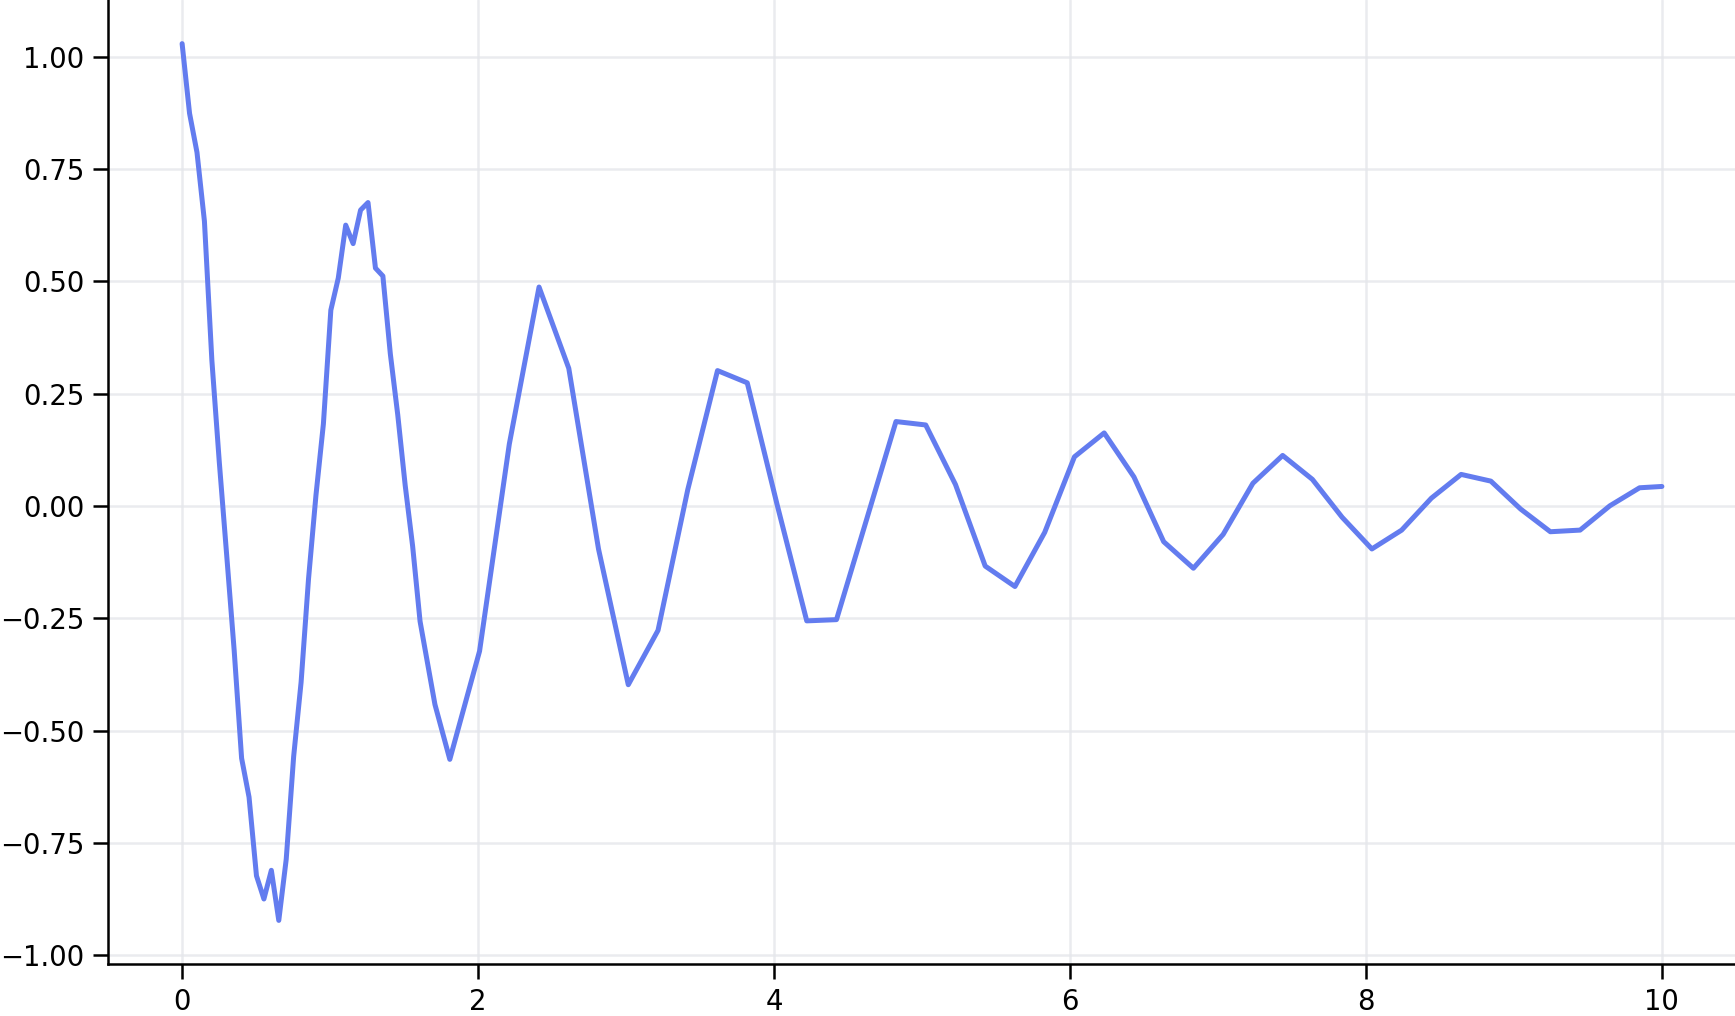
\includegraphics[width=.78\textwidth]{fig_plot_bad.png}
\caption{Risultato prodotto da \texttt{plot\_bad.py}.}
\end{figure}

\section{Rappresentare punti separati: \texttt{plot\_bad2.py}}
\begin{lstlisting}
import numpy as np
import matplotlib.pyplot as plt

dati = np.loadtxt("datios.txt")
x = dati[:, 0]
y = dati[:, 1]
plt.plot(x, y, "o")
plt.show()
\end{lstlisting}

La sola differenza rispetto allo script precedente è la stringa di formato \texttt{"o"}. Essa richiede marker circolari. Poiché non viene specificato uno stile di linea, i punti non sono collegati. Questa rappresentazione è più adatta quando si vogliono mostrare misure discrete senza suggerire che tra due punti consecutivi sia stata osservata una linea continua.

La stringa di formato può combinare colore, marker e stile della linea. Per esempio, \texttt{"ro-"} indica cerchi rossi collegati da una linea continua. È tuttavia spesso più leggibile usare argomenti espliciti, come \texttt{marker="o"}, \texttt{color="red"} e \texttt{linestyle="-"}.

\begin{figure}[H]
\centering
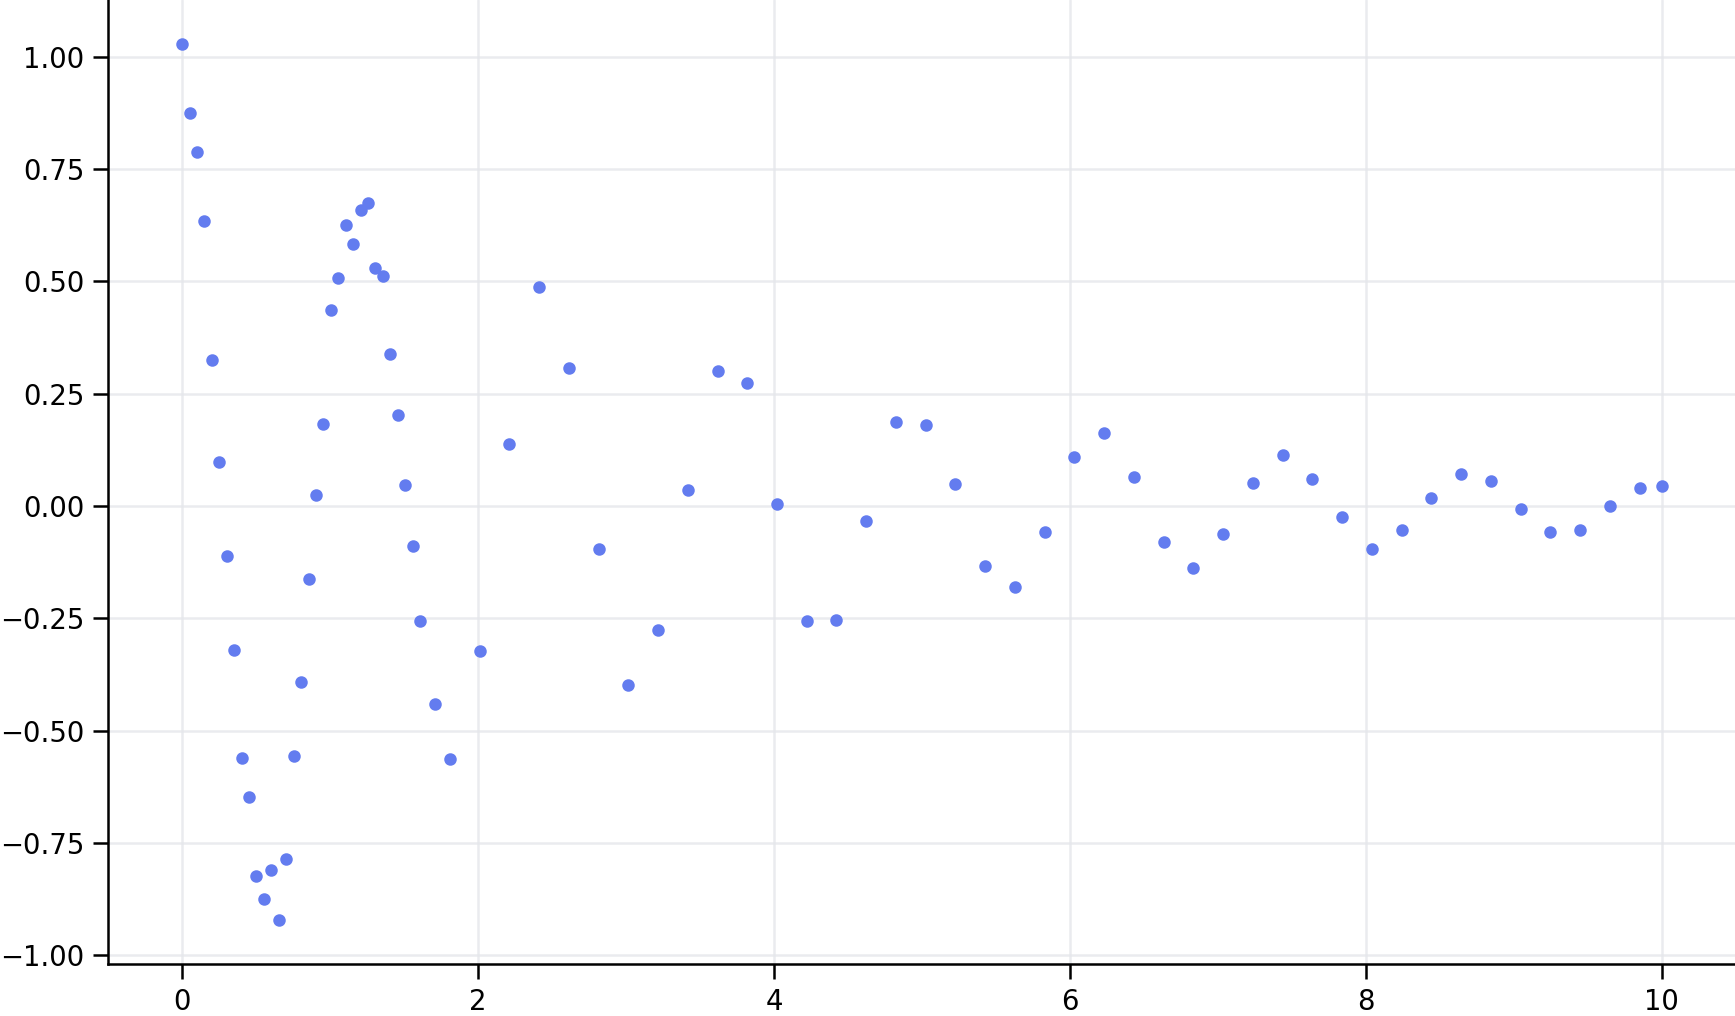
\includegraphics[width=.78\textwidth]{fig_plot_bad2.png}
\caption{Dati rappresentati mediante marker circolari.}
\end{figure}

\section{Etichetta e legenda: \texttt{plot\_bad3.py}}
\begin{lstlisting}
import numpy as np
import matplotlib.pyplot as plt

dati = np.loadtxt("datios.txt")
x = dati[:, 0]
y = dati[:, 1]
plt.plot(x, y, "^", label="Misure")
plt.legend()
plt.show()
\end{lstlisting}

Il marker \texttt{"\string^"} produce triangoli rivolti verso l'alto. L'argomento \texttt{label="Misure"} associa un nome all'oggetto grafico creato da \texttt{plot}. La chiamata \texttt{plt.legend()} raccoglie gli oggetti che possiedono una label e costruisce la legenda.

È importante distinguere i due passaggi: \texttt{label} definisce il testo associato alla serie, mentre \texttt{legend()} rende visibile la legenda. Se si omette \texttt{legend()}, la label rimane associata all'oggetto ma non viene mostrata.

\begin{figure}[H]
\centering
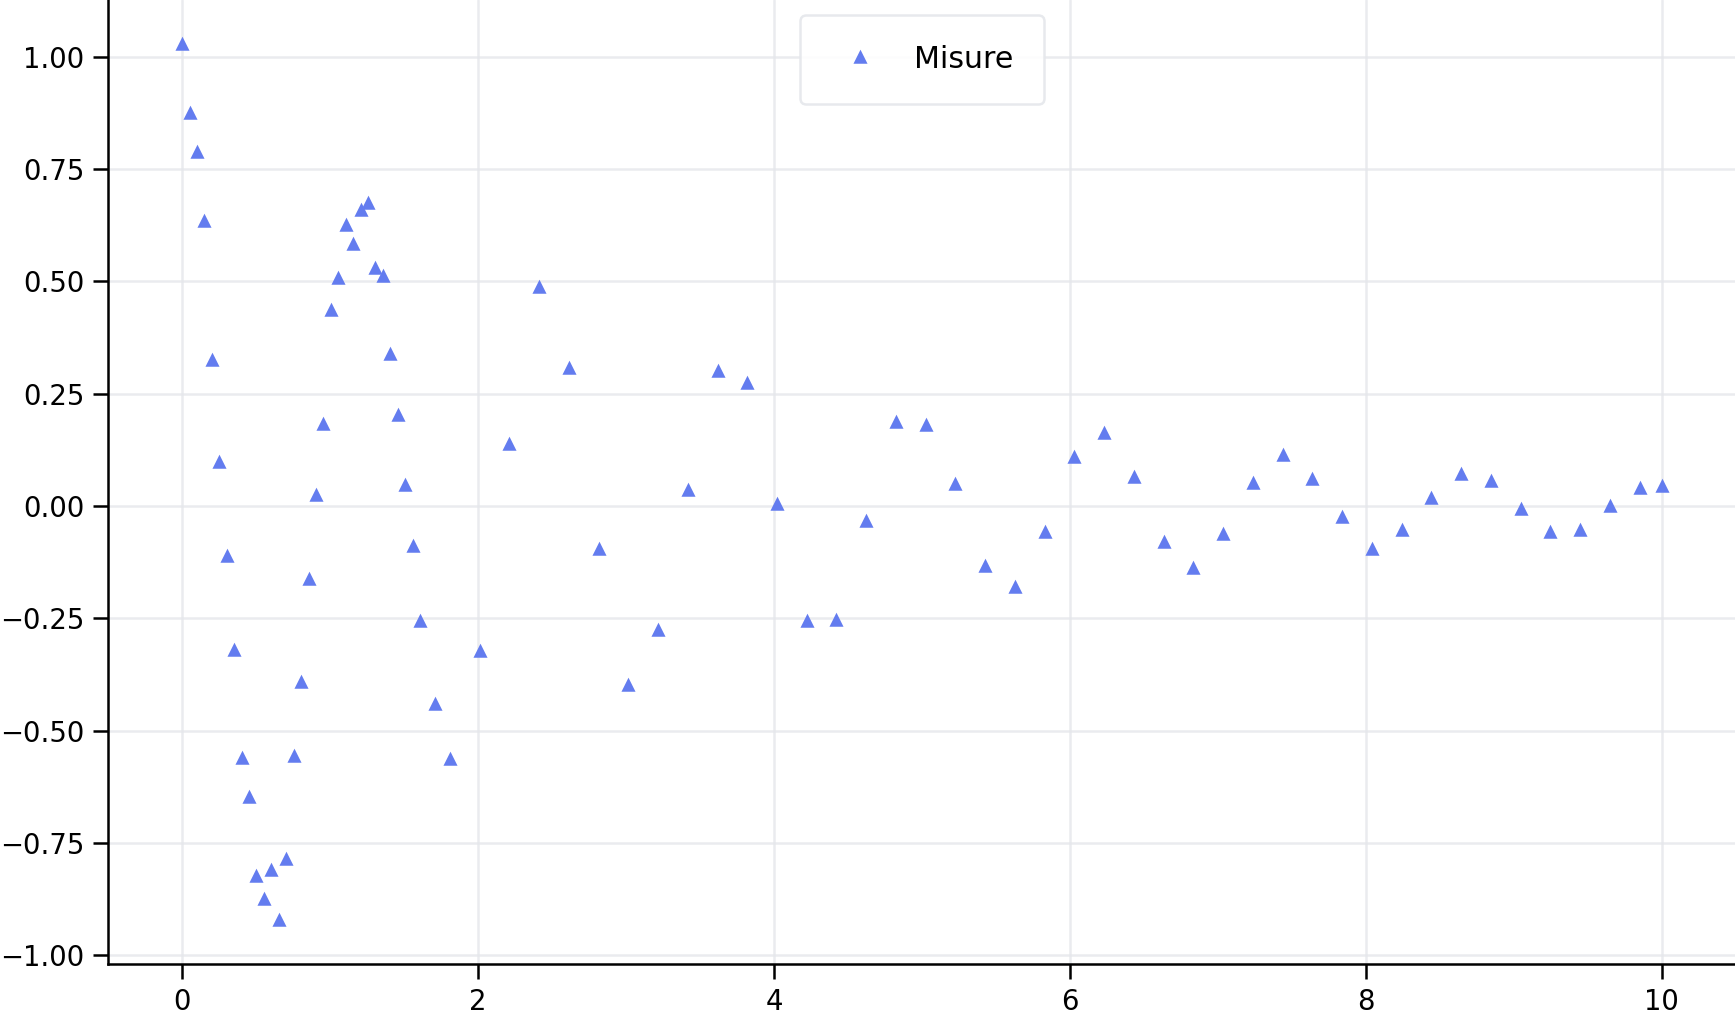
\includegraphics[width=.78\textwidth]{fig_plot_bad3.png}
\caption{Marker triangolari e legenda.}
\end{figure}

\section{Nomi e unità degli assi: \texttt{plot\_bad4.py}}
\begin{lstlisting}
import numpy as np
import matplotlib.pyplot as plt

dati = np.loadtxt("datios.txt")
x = dati[:, 0]
y = dati[:, 1]
plt.plot(x, y, "^", label="Misure")
plt.xlabel("Tempo (s)")
plt.ylabel("Distanza (cm)")
plt.legend()
plt.show()
\end{lstlisting}

Le funzioni \texttt{xlabel} e \texttt{ylabel} descrivono rispettivamente la grandezza riportata sull'asse orizzontale e quella riportata sull'asse verticale. In una figura scientifica si dovrebbero indicare sia il nome della grandezza sia l'unità di misura.

Il testo riportato sugli assi non modifica i dati e non esegue conversioni di unità. Se, per esempio, i dati fossero espressi in metri ma si volessero mostrare in centimetri, sarebbe necessario trasformare numericamente l'array prima del grafico.

\begin{figure}[H]
\centering
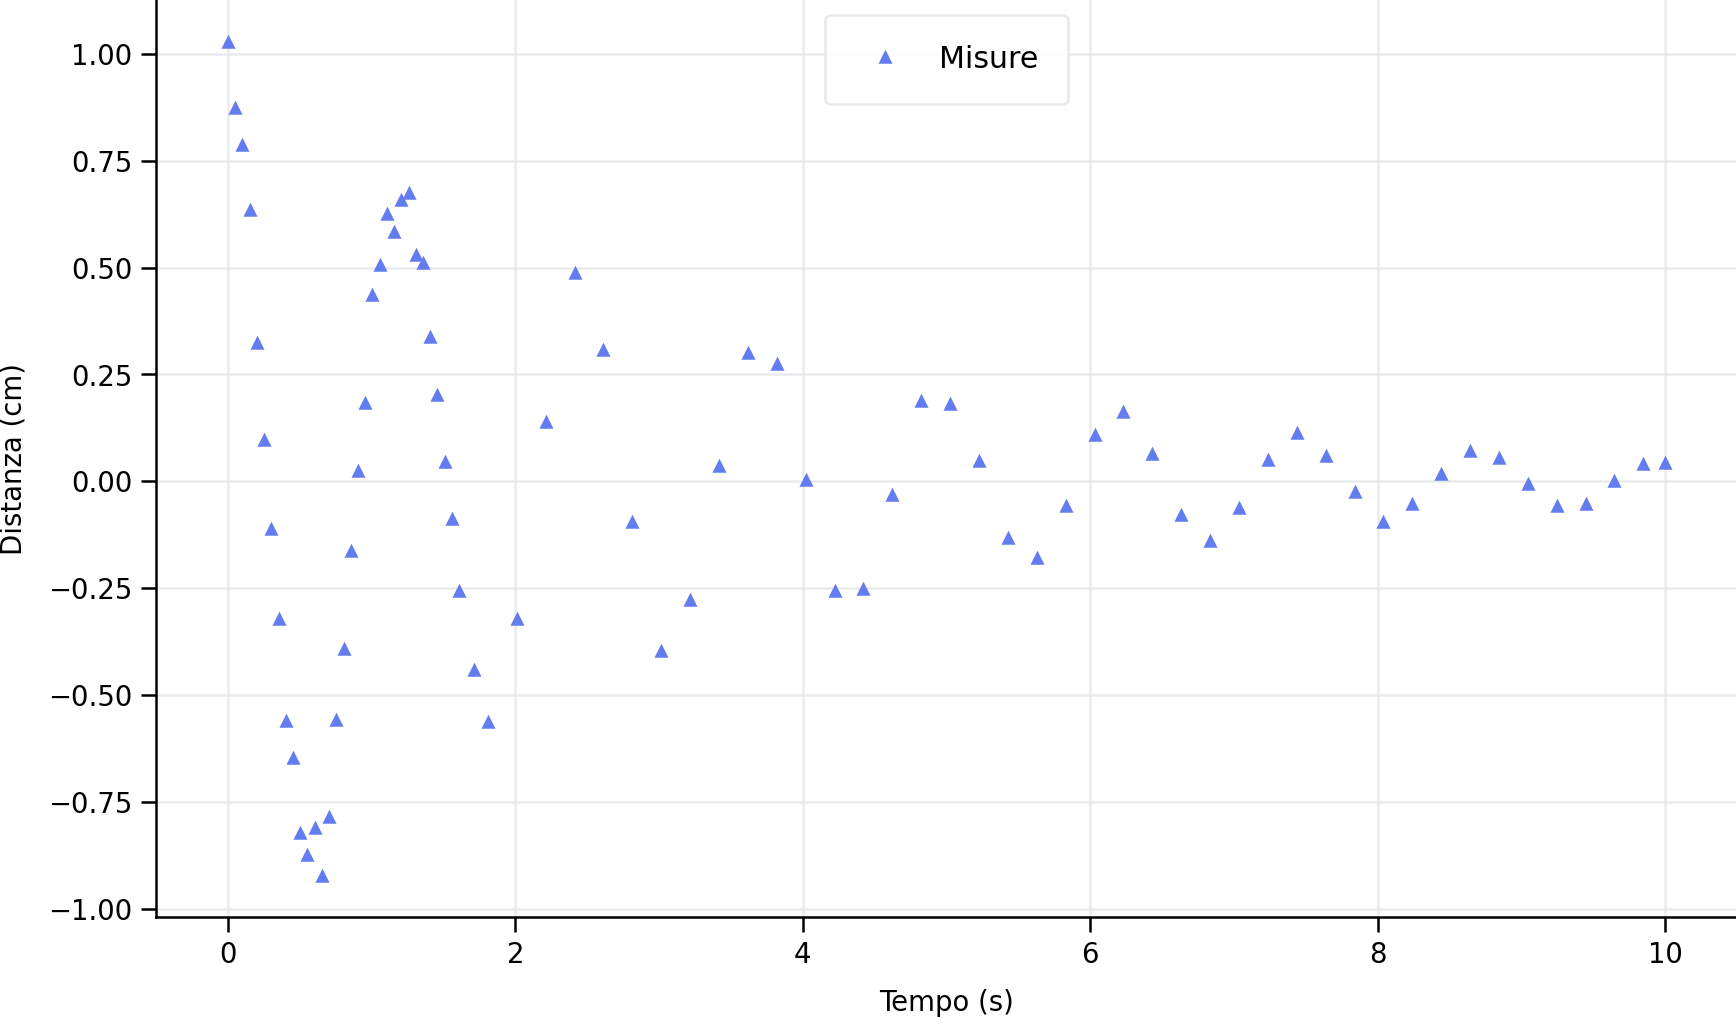
\includegraphics[width=.78\textwidth]{fig_plot_bad4.png}
\caption{Figura completa delle etichette degli assi.}
\end{figure}

\section{Due serie di dati: \texttt{plot\_bad5.py}}
\begin{lstlisting}
import numpy as np
import matplotlib.pyplot as plt

dati = np.loadtxt("Kter.txt")
x = dati[:, 0]
y1 = dati[:, 1]
y2 = dati[:, 2]

plt.plot(x, y1, "^", label="Misure 1")
plt.plot(x, y2, "o", label="Misure 2")
plt.xlabel("Distanza (cm)")
plt.ylabel("Frequenza (Hz)")
plt.legend()
plt.show()
\end{lstlisting}

Questo script legge tre colonne. La prima rappresenta la variabile indipendente comune alle due misure, mentre la seconda e la terza rappresentano due serie diverse. Le due chiamate a \texttt{plot} operano sugli stessi assi e sovrappongono le serie.

Marker e label differenti permettono di distinguere i due insiemi di dati anche quando i colori non sono facilmente riconoscibili. Questa scelta migliora la leggibilità nella stampa in scala di grigi e per utenti con difficoltà nella percezione dei colori.

\begin{figure}[H]
\centering
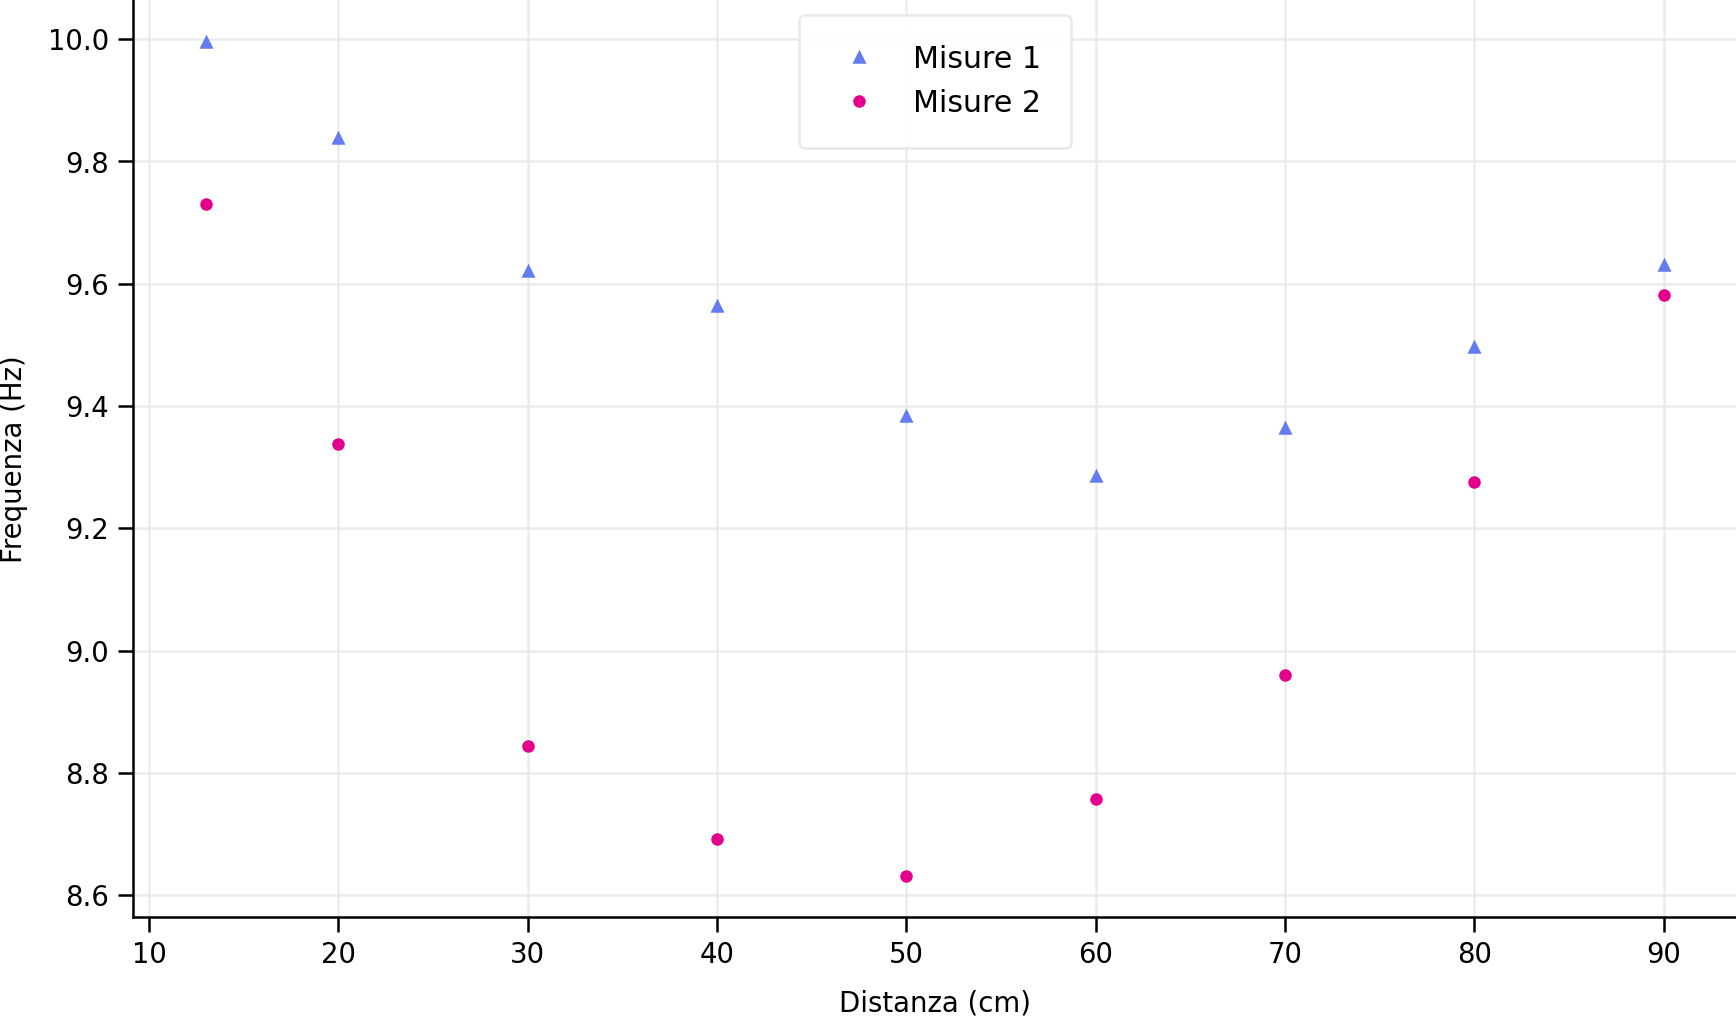
\includegraphics[width=.78\textwidth]{fig_plot_bad5.png}
\caption{Confronto tra due serie di misure.}
\end{figure}

\section{Lettura compatta e salvataggio: \texttt{plot\_bad6.py}}
\begin{lstlisting}
import numpy as np
import matplotlib.pyplot as plt

x, y1, y2 = np.loadtxt("Kter.txt", unpack=True)

plt.plot(x, y1, "^", label="Misure 1")
plt.plot(x, y2, "o", label="Misure 2")
plt.xlabel("Distanza (cm)")
plt.ylabel("Frequenza (Hz)")
plt.legend()

plt.savefig("grafico.pdf")
plt.savefig("grafico.png", dpi=300)
plt.show()
\end{lstlisting}

L'opzione \texttt{unpack=True} traspone concettualmente il risultato della lettura: le colonne vengono restituite come array separati e possono essere assegnate direttamente a \texttt{x}, \texttt{y1} e \texttt{y2}. Questo evita la selezione manuale mediante \texttt{dati[:, i]}.

Le due chiamate a \texttt{savefig} salvano la stessa figura in formati differenti:
\begin{itemize}
  \item il PDF conserva gli elementi grafici in forma vettoriale ed è particolarmente adatto a relazioni e pubblicazioni;
  \item il PNG è un formato raster; il parametro \texttt{dpi=300} richiede una risoluzione elevata, adatta alla stampa.
\end{itemize}

È opportuno salvare la figura prima di \texttt{show()}. Il comportamento di \texttt{show()} dipende dal backend e, in alcuni ambienti, la finestra può essere chiusa o la figura corrente può non essere più disponibile dopo la visualizzazione.

\begin{figure}[H]
\centering
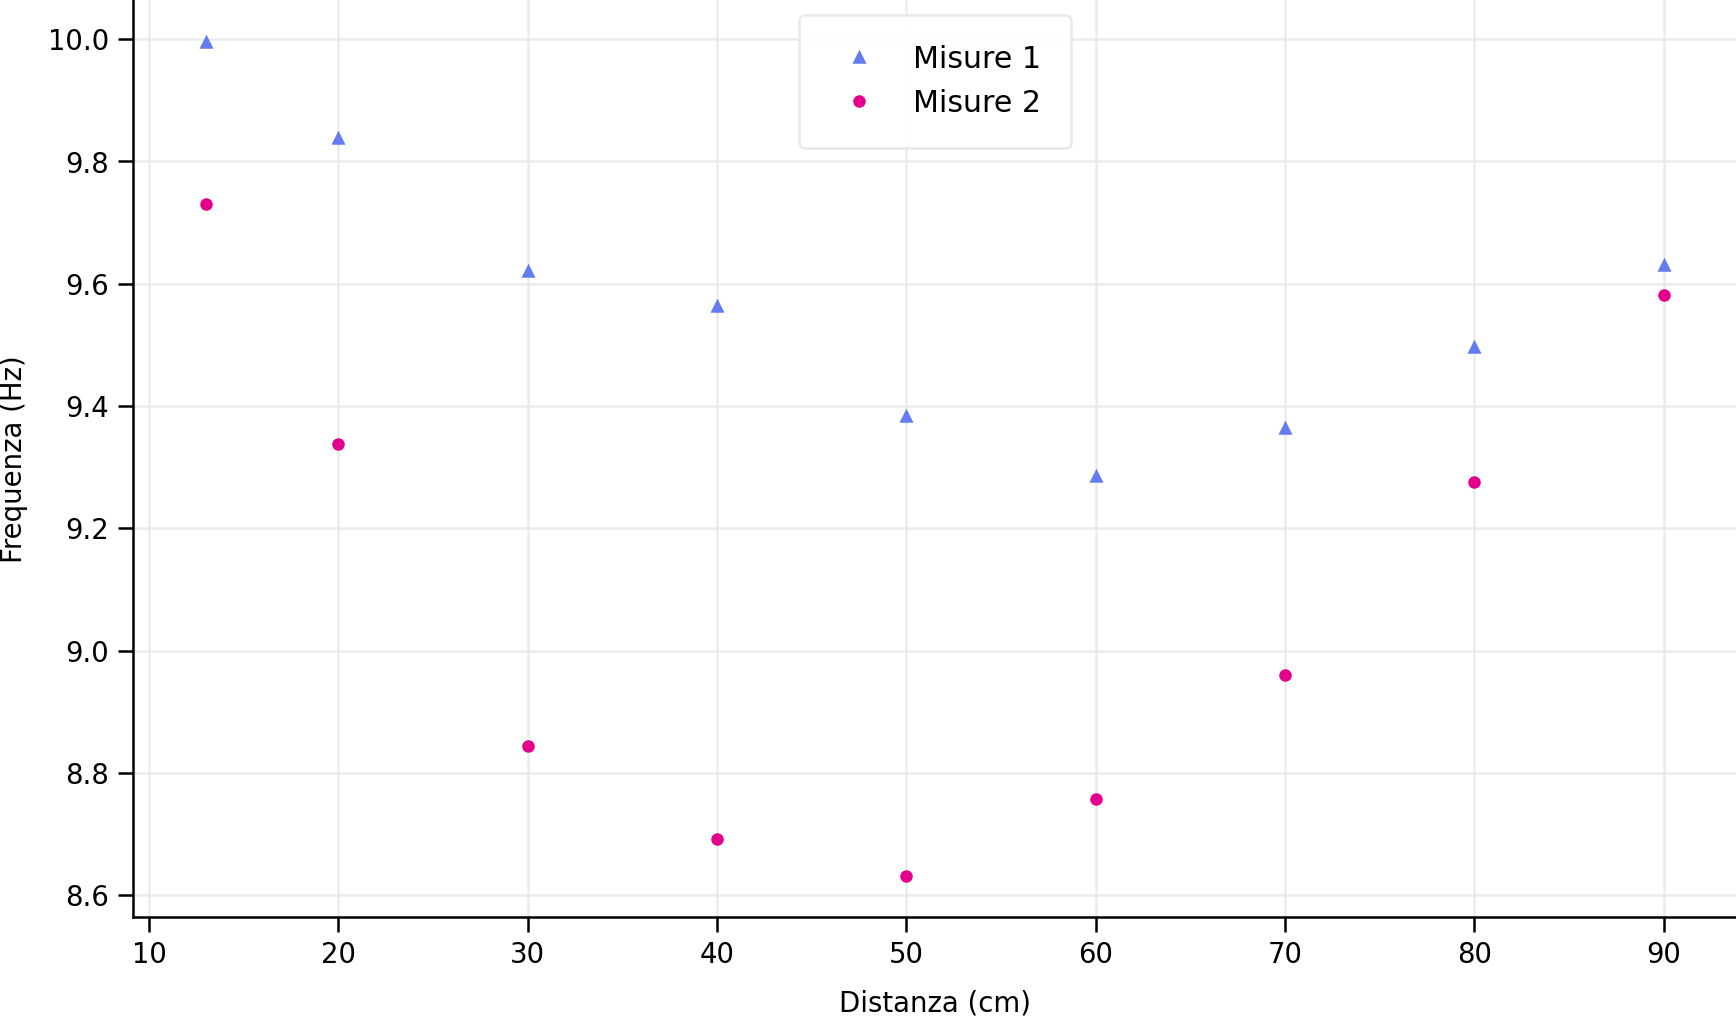
\includegraphics[width=.78\textwidth]{fig_plot_bad6.png}
\caption{Figura a due serie, pronta per essere salvata in PDF e PNG.}
\end{figure}

\section{Versione rifinita: \texttt{plottos2.py}}
\begin{lstlisting}
import numpy as np
import matplotlib.pyplot as plt
from matplotlib.ticker import MultipleLocator, AutoMinorLocator

# Lettura dati
x, y, xerr, yerr = np.loadtxt("datios.txt", unpack=True)

# Creazione figura
fig, ax = plt.subplots(figsize=(8, 6))

# Dati con barre di errore
ax.errorbar(
    x,
    y,
    xerr=xerr,
    yerr=yerr,
    fmt="o",
    color="blue",
    ecolor="gray",
    elinewidth=1,
    capsize=3,
    markersize=5,
    label="Misura",
)

# Etichette degli assi
ax.set_xlabel(
    "Tempo (s)",
    fontsize=24,
    fontweight="normal",
    fontname="Times",
)
ax.set_ylabel(
    "Distance (cm)",
    fontsize=24,
    fontweight="normal",
    fontname="Times",
)

# Tick principali
ax.tick_params(
    axis="both",
    which="major",
    labelsize=22,
    width=1.8,
    length=7,
    color="black",
)

# Tick secondari
ax.tick_params(
    axis="both",
    which="minor",
    width=1.2,
    length=4,
    color="black",
)

# Font dei valori numerici sugli assi
for label in ax.get_xticklabels() + ax.get_yticklabels():
    label.set_fontname("Times New Roman")

# Divisioni principali e secondarie
ax.xaxis.set_major_locator(MultipleLocator(1.0))
ax.yaxis.set_major_locator(MultipleLocator(0.5))
ax.xaxis.set_minor_locator(AutoMinorLocator(5))
ax.yaxis.set_minor_locator(AutoMinorLocator(5))

# Aspetto della cornice
for spine in ax.spines.values():
    spine.set_linewidth(1.3)
    spine.set_color("black")

# Legenda
ax.legend(
    loc="best",
    prop={"family": "Times New Roman", "size": 12},
)

# Layout finale
fig.tight_layout()
plt.show()
\end{lstlisting}

\subsection{Perché usare \texttt{fig} e \texttt{ax}}
La chiamata
\begin{lstlisting}
fig, ax = plt.subplots(figsize=(8, 6))
\end{lstlisting}
usa l'interfaccia orientata agli oggetti di Matplotlib. \texttt{fig} rappresenta il contenitore complessivo, cioè l'intera figura, mentre \texttt{ax} rappresenta il sistema di assi in cui vengono disegnati dati, etichette e legenda.

Questa impostazione è preferibile nei programmi articolati perché rende esplicito l'oggetto che si sta modificando. Inoltre, consente di gestire facilmente più pannelli nella stessa figura. \texttt{figsize=(8,6)} imposta larghezza e altezza in pollici; la forma $4:3$ è adatta a molte figure scientifiche.

\subsection{Barre di errore con \texttt{ax.errorbar}}
Gli argomenti \texttt{xerr=xerr} e \texttt{yerr=yerr} specificano le incertezze lungo gli assi orizzontale e verticale. Se gli array hanno la stessa lunghezza dei dati, ogni punto possiede la propria incertezza. Un singolo valore scalare, invece, assegnerebbe la stessa incertezza a tutti i punti.

Le principali opzioni grafiche sono:
\begin{description}[style=nextline]
  \item[\texttt{fmt="o"}] usa cerchi come marker e non aggiunge una linea tra i punti;
  \item[\texttt{color="blue"}] imposta il colore dei marker;
  \item[\texttt{ecolor="gray"}] imposta separatamente il colore delle barre di errore;
  \item[\texttt{elinewidth=1}] stabilisce lo spessore delle barre;
  \item[\texttt{capsize=3}] aggiunge piccoli segmenti terminali lunghi tre punti tipografici;
  \item[\texttt{markersize=5}] imposta la dimensione dei marker;
  \item[\texttt{label="Misura"}] assegna alla serie il testo usato dalla legenda.
\end{description}

\subsection{Etichette e caratteri}
I metodi \texttt{ax.set\_xlabel} e \texttt{ax.set\_ylabel} modificano le etichette del singolo oggetto \texttt{ax}. \texttt{fontsize=24} imposta la dimensione, \texttt{fontweight="normal"} il peso e \texttt{fontname} la famiglia tipografica.

Se il font richiesto non è installato, Matplotlib usa un font sostitutivo. Per ottenere un aspetto uniforme è opportuno usare la stessa famiglia per etichette, numeri degli assi e legenda. Nel codice è inoltre consigliabile uniformare la lingua, sostituendo eventualmente \texttt{Distance} con \texttt{Distanza}.

\subsection{Tick principali e secondari}
\texttt{tick\_params} controlla l'aspetto dei tick e delle relative etichette:
\begin{itemize}
  \item \texttt{axis="both"} applica le modifiche a entrambi gli assi;
  \item \texttt{which="major"} o \texttt{which="minor"} seleziona i tick principali o secondari;
  \item \texttt{labelsize} modifica la dimensione dei valori numerici;
  \item \texttt{width} imposta lo spessore dei tick;
  \item \texttt{length} ne imposta la lunghezza;
  \item \texttt{color} ne imposta il colore.
\end{itemize}

Le istruzioni con \texttt{MultipleLocator} stabiliscono il passo delle divisioni principali. Sull'asse $x$ un tick principale compare ogni $1.0$, mentre sull'asse $y$ compare ogni $0.5$. \texttt{AutoMinorLocator(5)} suddivide ciascun intervallo tra due tick principali in cinque parti uguali; di conseguenza, tra due tick principali compaiono quattro tick interni.

\subsection{Cornice, legenda e layout}
Gli elementi di \texttt{ax.spines} rappresentano i quattro lati della cornice. Il ciclo applica lo stesso spessore e lo stesso colore a tutti i lati.

In \texttt{ax.legend}, \texttt{loc="best"} lascia a Matplotlib la scelta della posizione che tende a sovrapporsi meno ai dati. L'argomento \texttt{prop} controlla famiglia e dimensione del carattere della legenda. Infine, \texttt{fig.tight\_layout()} ridistribuisce automaticamente gli spazi per ridurre il rischio che etichette o numeri vengano tagliati ai bordi.

\begin{figure}[H]
\centering
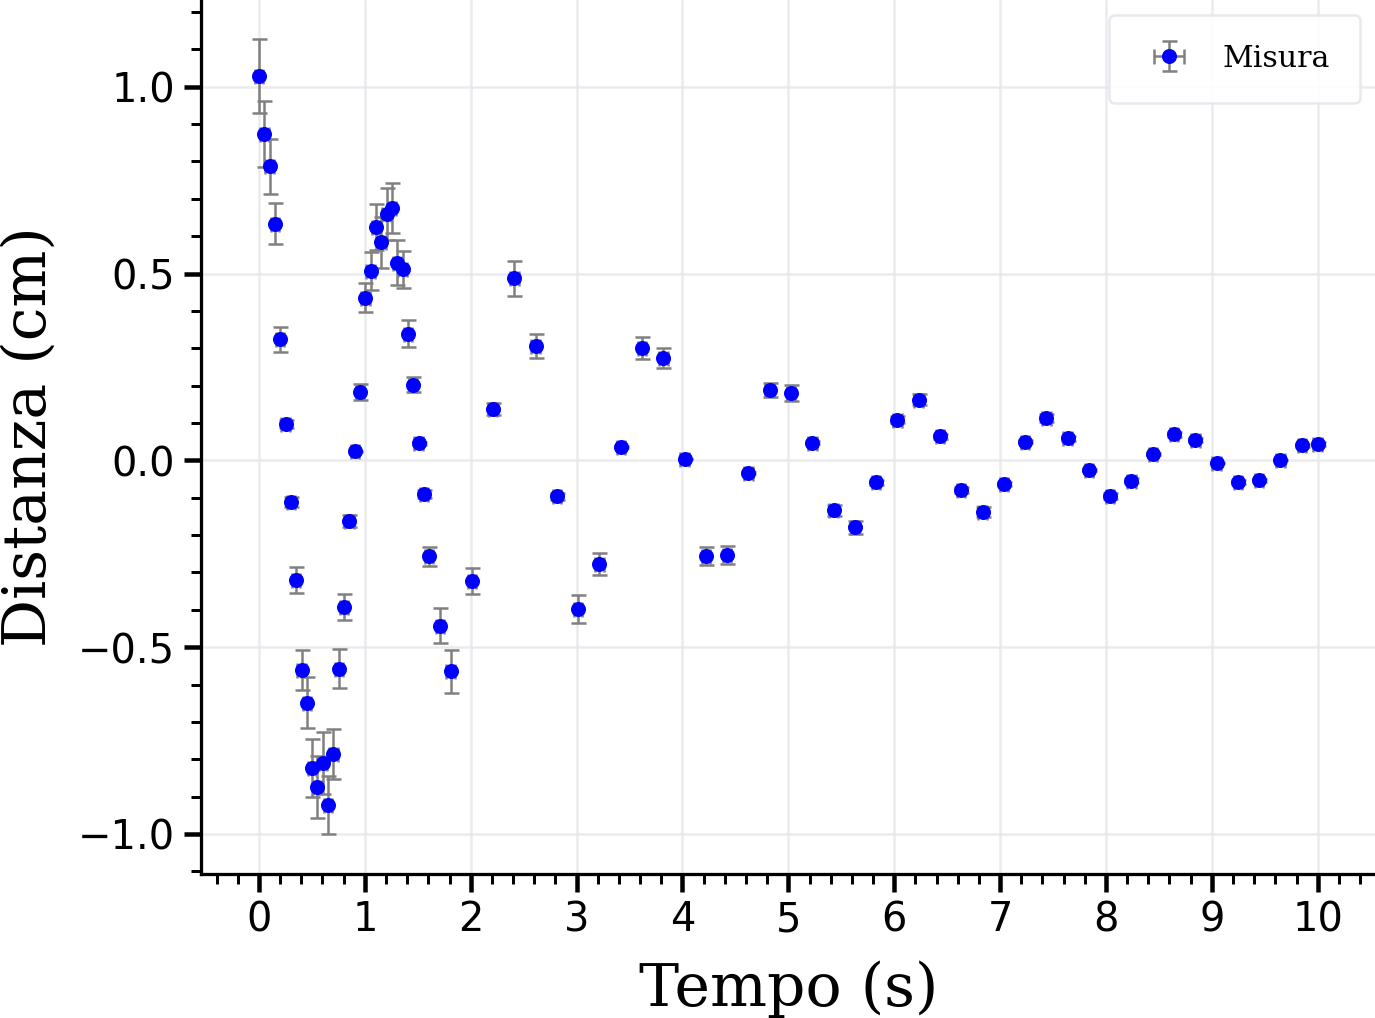
\includegraphics[width=.9\textwidth]{fig_plottos2.png}
\caption{Versione rifinita con barre di errore, tick principali e secondari e stile personalizzato.}
\end{figure}

\chapter{Fit parabolici con SciPy e NumPy}

\section{Problema matematico}
Gli script assumono che i dati possano essere descritti dal modello
\[
 f(x;a,b,c)=ax^2+bx+c.
\]
Per ogni punto sperimentale si definisce il residuo
\[
 r_i=y_i-f(x_i;a,b,c).
\]
Nel caso non pesato, il fit determina i parametri che minimizzano
\[
 S(a,b,c)=\sum_{i=1}^{N}r_i^2.
\]
Se sono note le incertezze $\sigma_i$ sulle ordinate, si minimizza invece il chi-quadro
\[
 \chi^2(a,b,c)=\sum_{i=1}^{N}
 \left[\frac{y_i-f(x_i;a,b,c)}{\sigma_i}\right]^2.
\]
Quando tutte le incertezze sono uguali, minimizzare il chi-quadro equivale, a meno di un fattore costante, a minimizzare la somma dei quadrati dei residui.

\section{Fit con \texttt{scipy.optimize.curve\_fit}}
\begin{lstlisting}
import numpy as np
import matplotlib.pyplot as plt
from scipy.optimize import curve_fit

# Funzione di fit
def parabola(x, a, b, c):
    return a*x**2 + b*x + c

# Lettura dati
x, y1, y2 = np.loadtxt("Kter.txt", unpack=True)

# Fit
popt1, pcov1 = curve_fit(parabola, x, y1)
popt2, pcov2 = curve_fit(parabola, x, y2)

# Errori sui parametri
perr1 = np.sqrt(np.diag(pcov1))
perr2 = np.sqrt(np.diag(pcov2))

# Griglia fitta per il disegno
xfit = np.linspace(np.min(x), np.max(x), 500)

plt.plot(x, y1, "^", label="Misure 1")
plt.plot(x, y2, "o", label="Misure 2")
plt.plot(xfit, parabola(xfit, *popt1),
         "r-", lw=2, label="Fit 1")
plt.plot(xfit, parabola(xfit, *popt2),
         "b-", lw=2, label="Fit 2")
plt.xlabel("Distanza (cm)")
plt.ylabel("Frequenza (Hz)")
plt.legend()
plt.savefig("grafico.pdf")
plt.savefig("grafico.png", dpi=300)
plt.show()
\end{lstlisting}

\subsection{Definizione del modello}
La funzione \texttt{parabola} riceve come primo argomento la variabile indipendente e, successivamente, i parametri da determinare. Questa struttura è richiesta da \texttt{curve\_fit}. Il vantaggio è che il modello non deve essere necessariamente un polinomio: può essere una funzione esponenziale, gaussiana, trigonometrica oppure una combinazione più complessa.

\subsection{Minimizzazione e chi-quadro}
\texttt{curve\_fit} esegue un fit ai minimi quadrati non lineari. Se \texttt{sigma} non viene specificato, il programma assume pesi uguali, equivalenti a un array di incertezze tutte unitarie, e minimizza la somma dei quadrati dei residui. Se si fornisce un array monodimensionale \texttt{sigma}, la funzione minimizzata è
\[
 \chi^2=\sum_i\left(\frac{r_i}{\sigma_i}\right)^2.
\]
Pertanto, è corretto descrivere \texttt{curve\_fit} come una procedura di minimizzazione del chi-quadro quando le incertezze sono esplicitamente fornite; senza \texttt{sigma}, si tratta del caso non pesato dello stesso schema.

Per un fit pesato si scrive:
\begin{lstlisting}
popt, pcov = curve_fit(
    parabola,
    x,
    y,
    sigma=yerr,
    absolute_sigma=True,
)
\end{lstlisting}
Con \texttt{absolute\_sigma=True}, le incertezze fornite sono interpretate in senso assoluto e la matrice di covarianza dei parametri mantiene questa normalizzazione. Con il valore predefinito \texttt{False}, conta inizialmente la scala relativa delle incertezze e la covarianza viene riscalata in relazione al chi-quadro ridotto ottenuto.

Per problemi senza vincoli, \texttt{curve\_fit} usa normalmente l'algoritmo di Levenberg--Marquardt. In presenza di limiti sui parametri passa a metodi compatibili con i vincoli, come il Trust Region Reflective. Nel caso della parabola il modello è lineare nei parametri $a$, $b$ e $c$, anche se \texttt{curve\_fit} viene utilizzato attraverso la sua interfaccia generale per fit non lineari.

\subsection{Parametri restituiti e operatore \texttt{*}}
\texttt{popt1} contiene i parametri ottimali nell'ordine con cui compaiono nella funzione:
\[
 \texttt{popt1}=[a,b,c].
\]
L'espressione \texttt{parabola(xfit, *popt1)} usa l'operatore di spacchettamento \texttt{*}: i tre elementi dell'array sono passati alla funzione come tre argomenti distinti.

\subsection{Costruzione della curva continua}
\texttt{np.linspace} genera 500 punti equidistanti tra il minimo e il massimo valore di $x$. Il fit viene valutato su questa griglia più fitta, non soltanto nei punti sperimentali. In questo modo la curva appare regolare. I dati restano rappresentati con marker, mentre il modello è mostrato con una linea continua di spessore \texttt{lw=2}.

\begin{figure}[H]
\centering
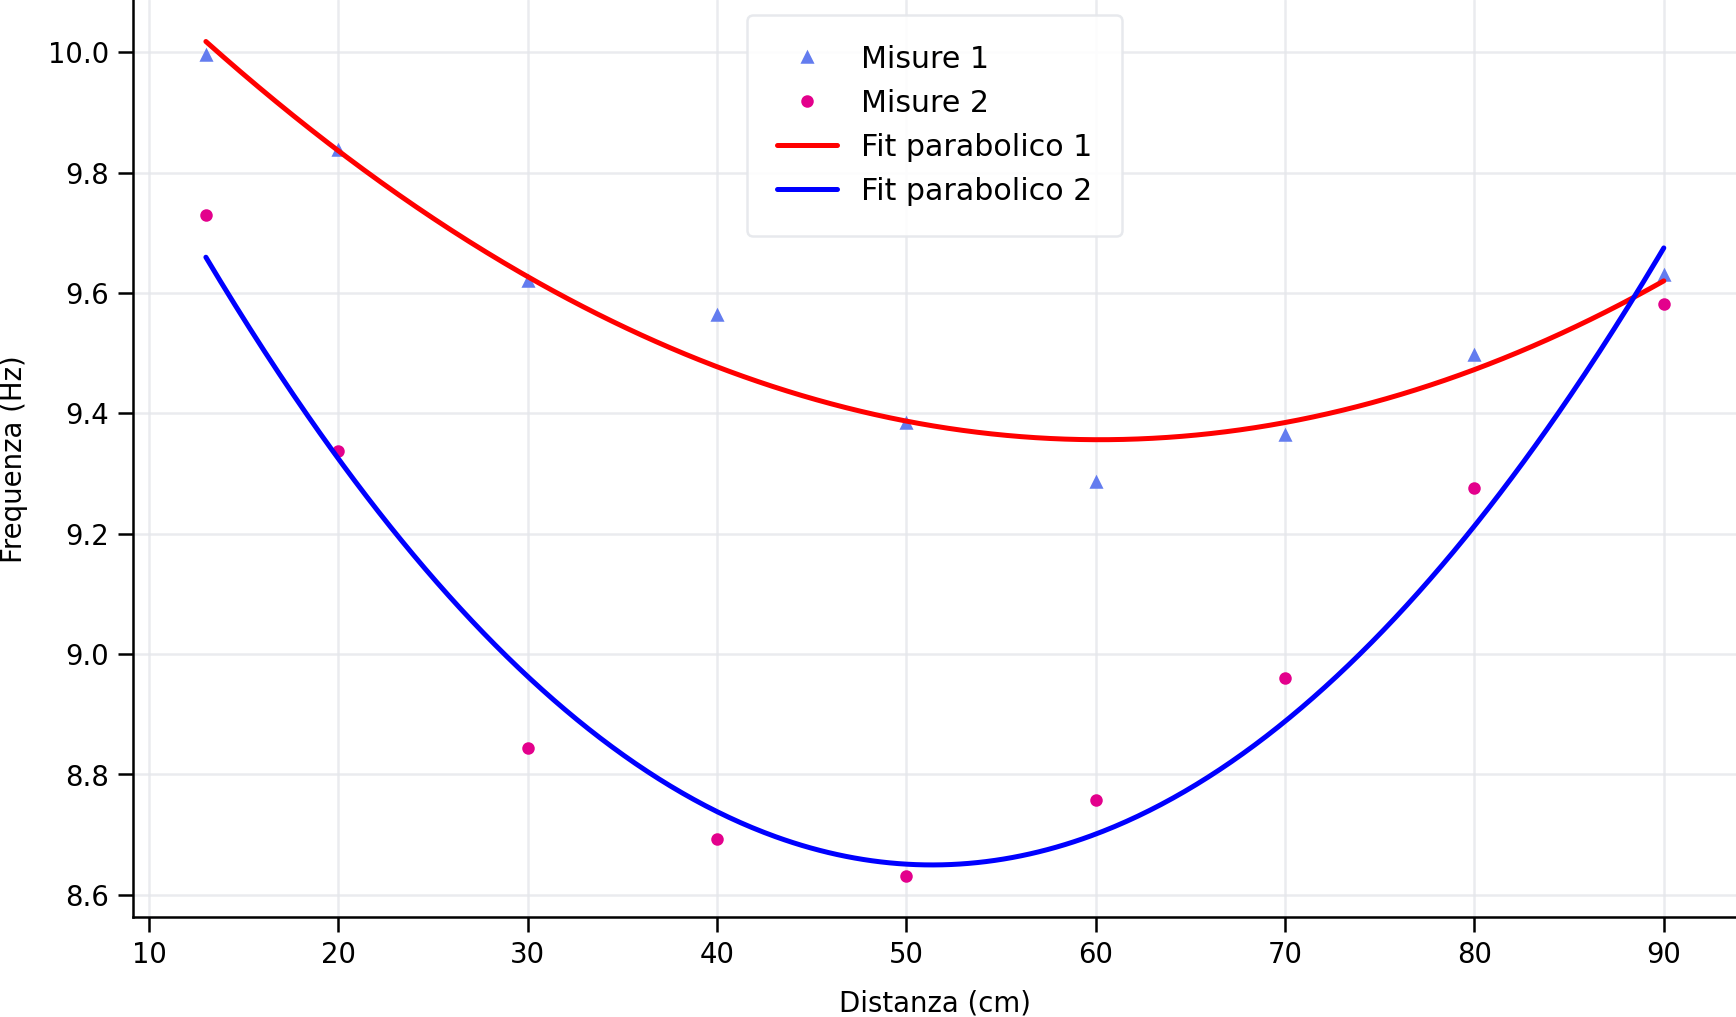
\includegraphics[width=.82\textwidth]{fig_fit_scipy.png}
\caption{Fit delle due serie mediante \texttt{scipy.optimize.curve\_fit}.}
\end{figure}

\section{Fit con \texttt{numpy.polyfit}}
\begin{lstlisting}
import numpy as np
import matplotlib.pyplot as plt

x, y1, y2 = np.loadtxt("Kter.txt", unpack=True)

# Fit quadratici
p1 = np.polyfit(x, y1, 2)
p2 = np.polyfit(x, y2, 2)

# Curva liscia per il disegno
xfit = np.linspace(x.min(), x.max(), 500)
yfit1 = np.polyval(p1, xfit)
yfit2 = np.polyval(p2, xfit)

plt.plot(x, y1, "^", label="Misure 1")
plt.plot(x, y2, "o", label="Misure 2")
plt.plot(xfit, yfit1, "r-", lw=2,
         label="Fit parabolico 1")
plt.plot(xfit, yfit2, "b-", lw=2,
         label="Fit parabolico 2")
plt.xlabel("Distanza (cm)")
plt.ylabel("Frequenza (Hz)")
plt.legend()
plt.savefig("grafico.pdf")
plt.savefig("grafico.png", dpi=300)
plt.show()
\end{lstlisting}

\subsection{Metodo dei minimi quadrati in NumPy}
\texttt{np.polyfit(x,y,2)} costruisce un polinomio di grado 2 e restituisce i coefficienti che minimizzano la somma dei quadrati dei residui. Il problema viene scritto nella forma matriciale
\[
 \mathbf{A}\mathbf{p}\simeq\mathbf{y},
\]
dove
\[
 \mathbf{A}=
 \begin{pmatrix}
 x_1^2 & x_1 & 1\\
 x_2^2 & x_2 & 1\\
 \vdots & \vdots & \vdots\\
 x_N^2 & x_N & 1
 \end{pmatrix},
 \qquad
 \mathbf{p}=
 \begin{pmatrix}a\\b\\c\end{pmatrix}.
\]
La matrice $\mathbf{A}$ è una matrice di Vandermonde. NumPy risolve il problema lineare ai minimi quadrati usando una decomposizione numerica collegata alla SVD, evitando di calcolare esplicitamente l'inversa di $\mathbf{A}^{T}\mathbf{A}$.

Il valore \texttt{2} è il grado del polinomio. I coefficienti sono ordinati dalla potenza più alta alla più bassa:
\[
 \texttt{p1[0]}=a,\qquad
 \texttt{p1[1]}=b,\qquad
 \texttt{p1[2]}=c.
\]
\texttt{np.polyval(p1,xfit)} valuta il polinomio nei punti della griglia \texttt{xfit}.

\subsection{Fit pesato con NumPy}
Se sono disponibili le incertezze $\sigma_i$ sulle ordinate, si può usare
\begin{lstlisting}
p = np.polyfit(x, y, 2, w=1/yerr)
\end{lstlisting}
I pesi di \texttt{polyfit} moltiplicano i residui non elevati al quadrato. Per ottenere il consueto chi-quadro, il peso corretto è quindi $w_i=1/\sigma_i$, non $1/\sigma_i^2$.

\section{Fit con NumPy e matrice di covarianza}
\begin{lstlisting}
import numpy as np
import matplotlib.pyplot as plt

x, y1, y2 = np.loadtxt("Kter.txt", unpack=True)

# Fit quadratici con matrice di covarianza
p1, cov1 = np.polyfit(x, y1, 2, cov=True)
p2, cov2 = np.polyfit(x, y2, 2, cov=True)

# Incertezze standard sui parametri
err1 = np.sqrt(np.diag(cov1))
err2 = np.sqrt(np.diag(cov2))

xfit = np.linspace(x.min(), x.max(), 500)
yfit1 = np.polyval(p1, xfit)
yfit2 = np.polyval(p2, xfit)

plt.plot(x, y1, "^", label="Misure 1")
plt.plot(x, y2, "o", label="Misure 2")
plt.plot(xfit, yfit1, "r-", lw=2,
         label="Fit parabolico 1")
plt.plot(xfit, yfit2, "b-", lw=2,
         label="Fit parabolico 2")
plt.xlabel("Distanza (cm)")
plt.ylabel("Frequenza (Hz)")
plt.legend()

print("\nFit 1")
print(f"a = {p1[0]:.5g} +/- {err1[0]:.2g}")
print(f"b = {p1[1]:.5g} +/- {err1[1]:.2g}")
print(f"c = {p1[2]:.5g} +/- {err1[2]:.2g}")

print("\nFit 2")
print(f"a = {p2[0]:.5g} +/- {err2[0]:.2g}")
print(f"b = {p2[1]:.5g} +/- {err2[1]:.2g}")
print(f"c = {p2[2]:.5g} +/- {err2[2]:.2g}")

plt.savefig("grafico.pdf")
plt.savefig("grafico.png", dpi=300)
plt.show()
\end{lstlisting}

\section{Significato della matrice di covarianza}
La matrice di covarianza dei parametri è, nel caso di tre parametri,
\[
 \mathbf{C}=
 \begin{pmatrix}
 \operatorname{Var}(a) & \operatorname{Cov}(a,b) & \operatorname{Cov}(a,c)\\
 \operatorname{Cov}(b,a) & \operatorname{Var}(b) & \operatorname{Cov}(b,c)\\
 \operatorname{Cov}(c,a) & \operatorname{Cov}(c,b) & \operatorname{Var}(c)
 \end{pmatrix}.
\]
Essa descrive sia le incertezze individuali dei parametri sia le loro correlazioni statistiche.

Gli elementi diagonali sono le varianze stimate:
\[
 C_{aa}=\sigma_a^2,\qquad
 C_{bb}=\sigma_b^2,\qquad
 C_{cc}=\sigma_c^2.
\]
Per questo motivo le incertezze standard si ricavano mediante
\begin{lstlisting}
err = np.sqrt(np.diag(cov))
\end{lstlisting}
Gli elementi fuori diagonale sono covarianze. Una covarianza diversa da zero indica che le variazioni ammissibili di due parametri non sono indipendenti. In un fit parabolico, per esempio, una variazione del coefficiente quadratico può essere parzialmente compensata da una variazione del coefficiente lineare o del termine costante.

La matrice è utile per:
\begin{itemize}
  \item riportare correttamente le incertezze sui parametri;
  \item valutare le correlazioni tra i parametri;
  \item propagare le incertezze a una quantità dipendente dai parametri;
  \item costruire bande di incertezza della funzione di fit;
  \item riconoscere fit mal condizionati, nei quali alcuni parametri risultano fortemente correlati.
\end{itemize}

La correlazione normalizzata tra due parametri $p_i$ e $p_j$ è
\[
 \rho_{ij}=\frac{C_{ij}}{\sqrt{C_{ii}C_{jj}}},
\]
con valori compresi tra $-1$ e $+1$. Valori in modulo vicini a uno indicano una forte correlazione o anticorrelazione.

In \texttt{np.polyfit(...,cov=True)}, la covarianza è normalmente scalata in modo che il chi-quadro ridotto sia unitario. Se si forniscono pesi derivati da incertezze assolute affidabili, si può richiedere
\begin{lstlisting}
p, cov = np.polyfit(
    x, y, 2,
    w=1/yerr,
    cov="unscaled",
)
\end{lstlisting}
In \texttt{curve\_fit}, il ruolo analogo è svolto dall'opzione \texttt{absolute\_sigma=True}.

\section{Propagazione della covarianza alla curva di fit}
Il valore della parabola in un punto $x$ può essere scritto come
\[
 f(x)=\mathbf{v}^{T}\mathbf{p},
 \qquad
 \mathbf{v}=\begin{pmatrix}x^2\\x\\1\end{pmatrix}.
\]
La varianza propagata della curva è
\[
 \sigma_f^2(x)=\mathbf{v}^{T}\mathbf{C}\mathbf{v}.
\]
In Python si può calcolare una banda di incertezza con:
\begin{lstlisting}
V = np.column_stack((xfit**2, xfit, np.ones_like(xfit)))
var_fit = np.einsum("ij,jk,ik->i", V, cov1, V)
sigma_fit = np.sqrt(var_fit)

plt.fill_between(
    xfit,
    yfit1 - sigma_fit,
    yfit1 + sigma_fit,
    alpha=0.25,
    label="Incertezza del fit",
)
\end{lstlisting}
Questa banda rappresenta l'incertezza associata ai parametri stimati e alle loro covarianze. Non coincide necessariamente con un intervallo di previsione per una nuova misura, che dovrebbe includere anche la dispersione sperimentale dei singoli dati.

\section{Confronto tra NumPy e SciPy}
\begin{center}
\begin{tabular}{p{.22\textwidth}p{.34\textwidth}p{.34\textwidth}}
\toprule
Aspetto & \texttt{numpy.polyfit} & \texttt{scipy.optimize.curve\_fit}\\
\midrule
Tipo di modello & Polinomio di grado assegnato & Funzione Python generica\\
Problema numerico & Minimi quadrati lineari nei coefficienti & Minimi quadrati non lineari in forma generale\\
Funzione obiettivo & Somma dei quadrati, eventualmente pesata & Chi-quadro con \texttt{sigma}; caso non pesato se \texttt{sigma=None}\\
Valori iniziali & Non richiesti & Utili o necessari per modelli non lineari complessi\\
Risultato & Coefficienti polinomiali & Parametri nell'ordine della funzione\\
Covarianza & Con \texttt{cov=True} & Restituita come \texttt{pcov}\\
Pesi & \texttt{w=1/sigma} & \texttt{sigma=sigma}\\
Uso tipico & Regressioni polinomiali & Modelli generici, anche non lineari\\
\bottomrule
\end{tabular}
\end{center}

È importante non contrapporre rigidamente ``minimi quadrati'' e ``chi-quadro'': il chi-quadro è una somma di residui quadratici normalizzati dalle incertezze. NumPy e SciPy appartengono quindi alla stessa famiglia concettuale. La differenza principale è che \texttt{polyfit} sfrutta la linearità del polinomio rispetto ai coefficienti e risolve direttamente un problema lineare, mentre \texttt{curve\_fit} usa un algoritmo iterativo generale per minimizzare la funzione obiettivo.

Nel caso della parabola e in assenza di pesi, i due metodi devono fornire risultati compatibili entro la precisione numerica. Le differenze diventano sostanziali quando il modello non è lineare nei parametri, quando si introducono vincoli oppure quando sono necessari valori iniziali.

\section{Stampa corretta dei parametri}
La sintassi
\begin{lstlisting}
print(f"a = {p1[0]:.5g} +/- {err1[0]:.2g}")
\end{lstlisting}
usa una f-string. L'espressione \texttt{p1[0]} seleziona il parametro, mentre \texttt{:.5g} richiede cinque cifre significative. Analogamente, \texttt{:.2g} richiede due cifre significative per l'incertezza.

Non devono comparire backslash all'interno delle parentesi quadre della f-string. Forme come \texttt{p1\textbackslash[0\textbackslash]} producono un errore sintattico. Inoltre, il formato deve essere applicato all'elemento dell'array e non all'array stesso.

\begin{figure}[H]
\centering
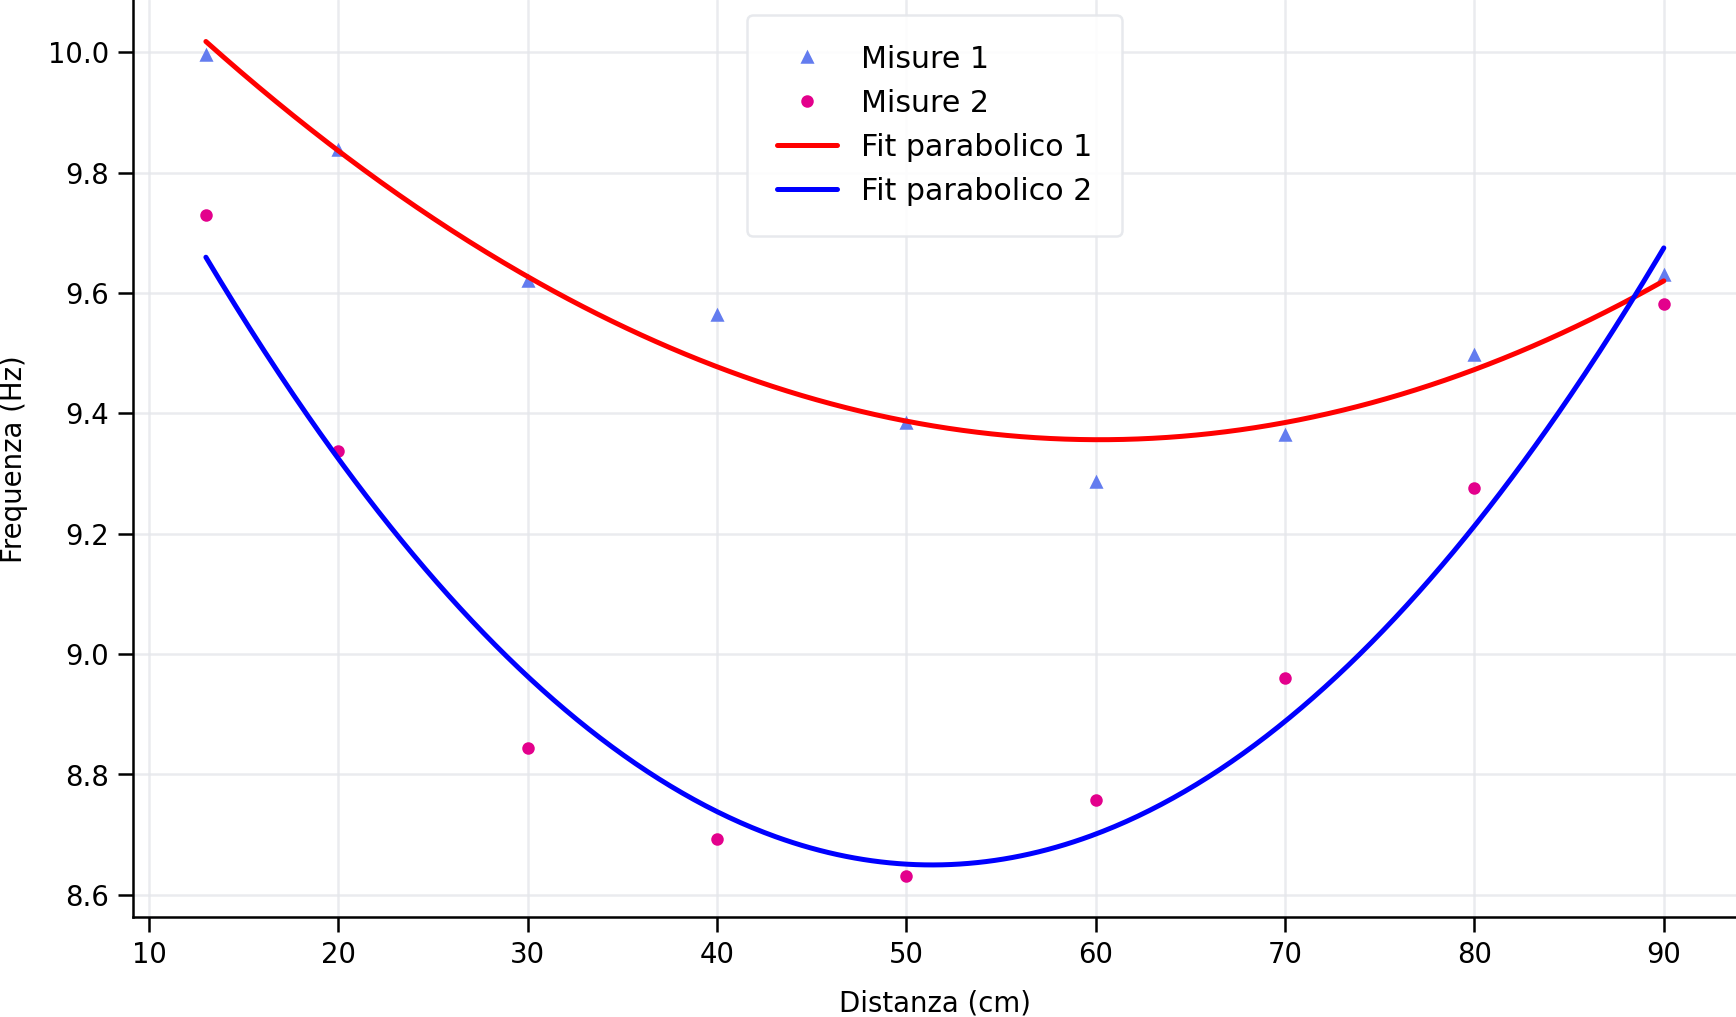
\includegraphics[width=.82\textwidth]{fig_fit_numpy.png}
\caption{Fit parabolico ottenuto con \texttt{numpy.polyfit} e valutato con \texttt{numpy.polyval}.}
\end{figure}

\chapter{Buone pratiche conclusive}
\begin{itemize}
  \item mantenere coerenti i nomi dei file negli script e nella cartella di lavoro;
  \item indicare sempre grandezze e unità sugli assi;
  \item distinguere serie diverse mediante marker oltre che mediante colori;
  \item usare l'interfaccia \texttt{fig, ax} per figure complesse o con più pannelli;
  \item rappresentare le incertezze sperimentali quando sono disponibili;
  \item salvare la figura prima di chiamare \texttt{show()};
  \item usare PDF per la grafica vettoriale e PNG ad alta risoluzione per la grafica raster;
  \item usare un fit pesato quando le incertezze dei punti non sono uguali;
  \item riportare parametri, incertezze, covarianze e un indicatore della qualità del fit;
  \item controllare i residui, perché un valore accettabile del chi-quadro non sostituisce l'ispezione dell'andamento sistematico degli scarti.
\end{itemize}

\end{document}
